\RequirePackage{plautopatch}
\documentclass[upLaTeX,a4paper]{jsarticle}
\usepackage{listings,jlisting,amsmath,otf,here}
\usepackage[dvipdfmx]{graphicx}

\lstset{
breaklines = true,
numbers = left,
frame = tbrl,
tabsize = 4,
captionpos = t
}

\title{流体の数値計算プログラムの作成 中間報告}
\author{B4 津田修一朗}
\date{}

\begin{document}
\maketitle

\section{これまでに取り組んだこと}
\subsection{環境構築}
gfortranとgnuplotをインストールした.
エディタはVisual Studio Codeを使用している.

\subsection{流れ関数と渦度を求めるプログラムの実装}
流れ関数-渦度法により,cavity内の流れを解いた.基礎方程式については,資料「流体の数値計算(川口光年先生1976年頃).pdf」に従った.レイノルズ数$Re = 50$, 格子点$50\times 50$とした.

\subsection{速度ベクトル図の描画}
流れ関数と渦度を求めるプログラムの実装により得られた流れ関数$\phi$より,速度場$(u, v)$を

\begin{equation}
  u = \frac{\partial \phi}{\partial y}, v = - \frac{\partial \phi}{\partial x},
\end{equation}
を用いて求めた.
その結果は図\ref{fig:velocity_vector}の通りである.
\begin{figure}[H]
  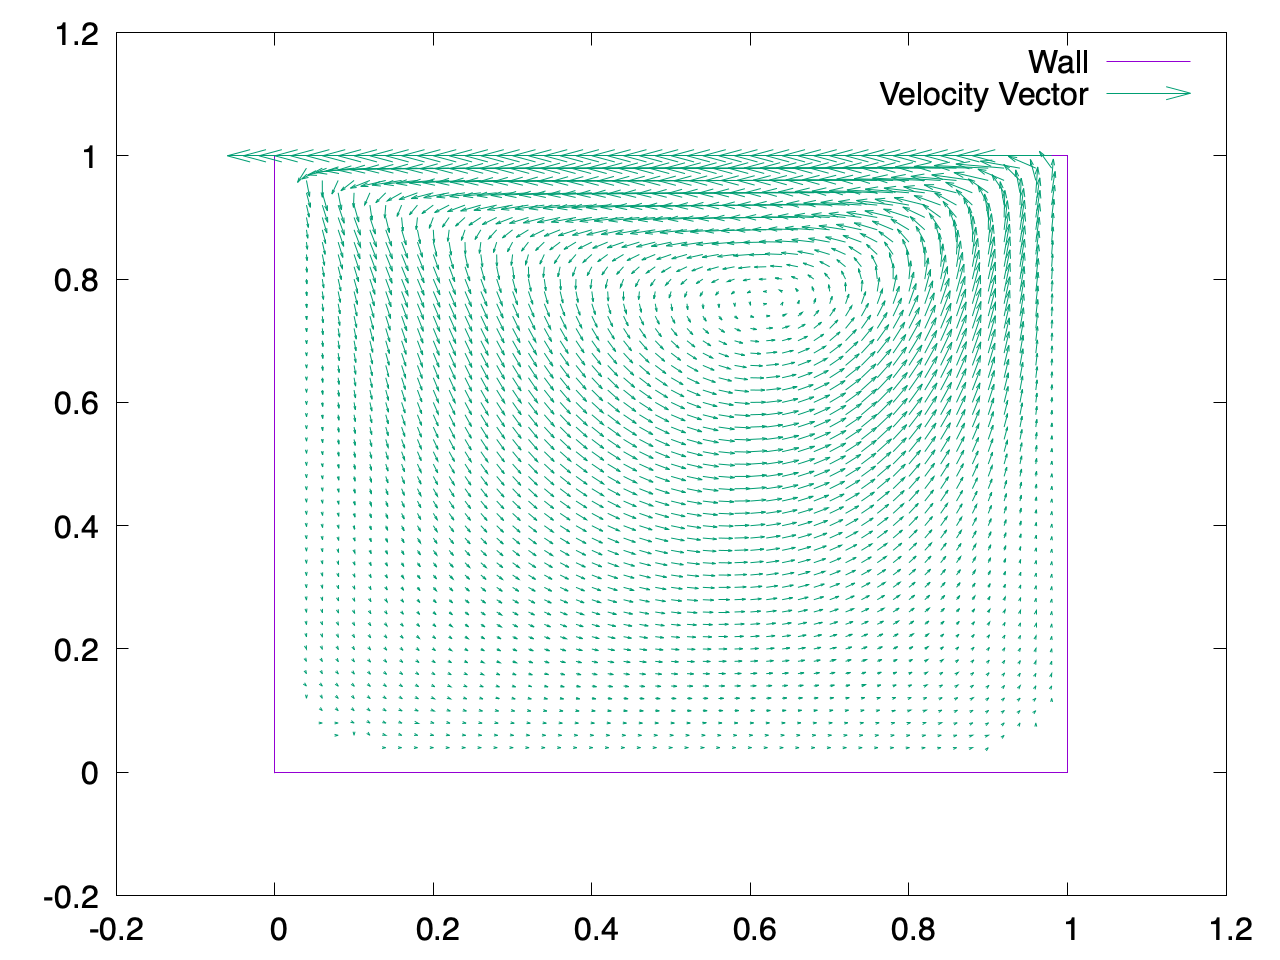
\includegraphics[width=15cm]{outputs/img/velocity_vector_50.png}
  \caption{速度ベクトル}
  \label{fig:velocity_vector}
\end{figure}

\section{現在取り組んでいること}
\subsection*{流線図の描画}
流線は流れ関数$\phi = const$で表されることを用いて、流れ関数と渦度を求めるプログラムにより求めた流れ関数を用いて流線図の描画を行った。
その結果を図\ref{fig:stream_line_50}に示す。図\ref{fig:stream_line_50}において、描画に用いる点の数が格子点数に比べて少ないため、曲線による補完や格子点の数を増やすことを検討している。
\begin{figure}[H]
  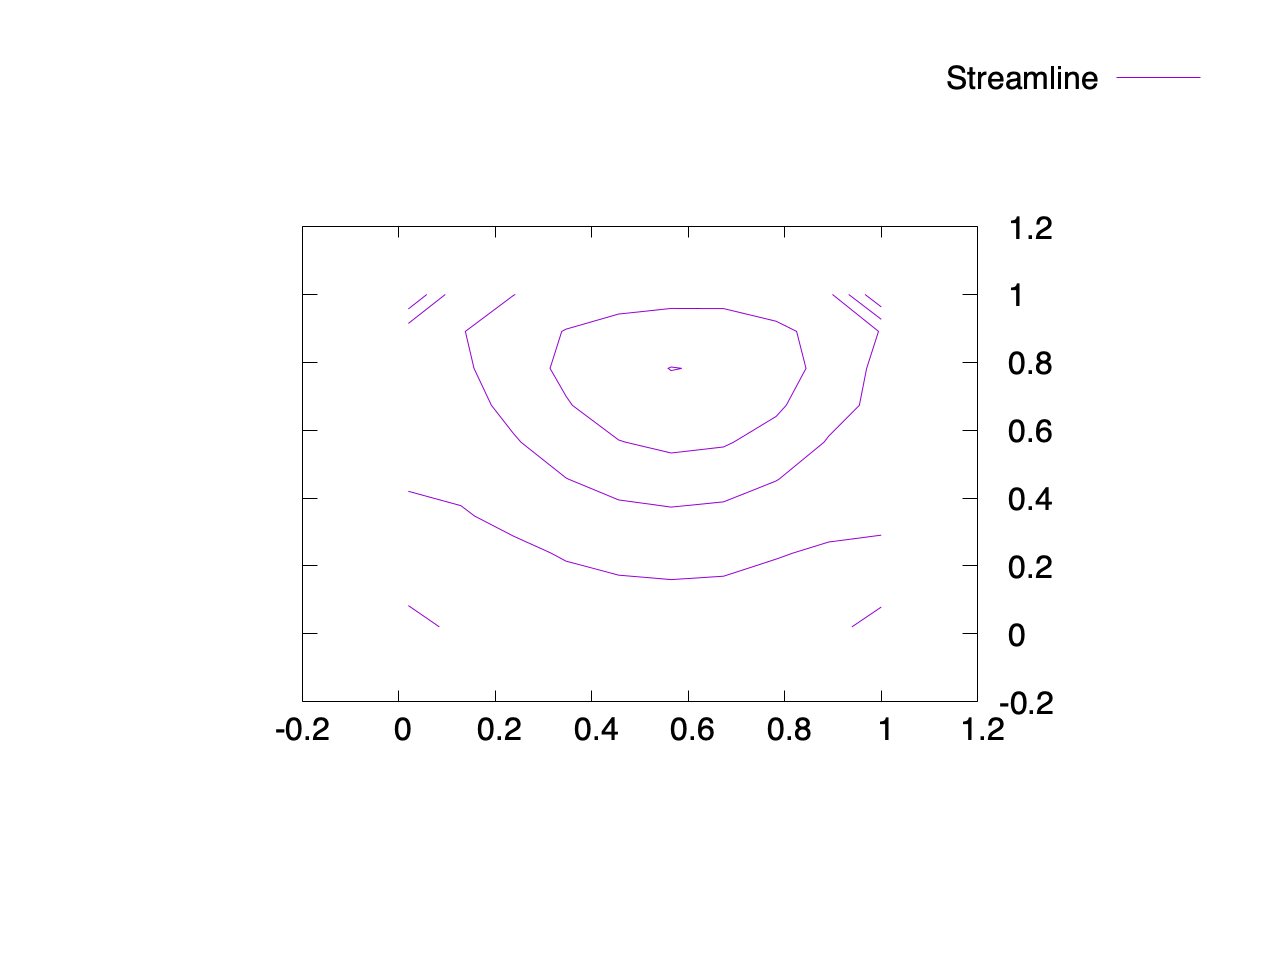
\includegraphics[width=15cm]{outputs/img/stream_line_50.png}
  \caption{流線}
  \label{fig:stream_line_50}
\end{figure}
\section{これから取り組むこと}
\subsection{等圧線図の描画}
圧力のポアソン方程式等により圧力分布を求め、等圧線図を描画する.

\subsection{リファクタリング}
同じ処理を複数回記述している箇所があるので、関数、モジュールを用いることができるか検討する。


\end{document}